\section{Spørgsmål 9}

% Hvad er Databasetransaktioner i en relationel database, kom herunder ind på ACID egenskaber samt betydningen af låse og låsning.

\subsection{Fokuspunkter}
\begin{itemize}
	\item Hvad er Databasetransaktioner i en relationel database?
	\begin{itemize}
		\item Kom herunder ind på ACID egenskaber.
		\item Samt betydningen af låse og låsning.
	\end{itemize}
\end{itemize}

\subsection{Litteratur}
\begin{itemize}
	
%	\item Fra teori: Database Modeling and Design. Logical Design 5'th Ed.
%	\begin{itemize}
%		\item Ch. 1 (p1 - 11)
%		\item Ch. 2 (p13 - 34)
%		\item Ch. 3 (p35 - 53)
%		\item Ch. 4 (p55 - 84)
%	\end{itemize}
	
	\item Fra Database eLearning: \url{http://db.grussell.org/index.html}.
	\begin{itemize}
		\item Ch 6 Concurrency, Transacttions and Implementations.
		\begin{itemize}
			\item Concurrency using Transactions.
			\item Concurrency.
		\end{itemize}
	\end{itemize}
	
	\item Fra wikipedia:
	\begin{itemize}
		\item \href{https://en.wikipedia.org/wiki/Database_transaction}{Database transaction}
		\item \href{https://en.wikipedia.org/wiki/ACID}{ACID}
	\end{itemize}
	
%	\item Fra Agile Data Home Page:
%	\begin{itemize}
%		\item 
%	\end{itemize}
\end{itemize}

\newpage

% must
\subsection{Hvad er Databasetransaktioner i en relationel database?}
En databasetransaktion er en række operationer der udføres samlet i DBMS. Database transaktioner bruges til at samle flere mindre opgaver og udføre dem atomic, consistent, isolated og durable (ACID). En database transaktion skal:

\begin{itemize}
	\item Ske uden at forstyrre andre transaktioner (må ikke interferere)
	\item Den data der tilgås skal også kunne bruges af andre klienter samtidig.
\end{itemize}

Et eksempel på en Database transaktion kunne være en bank transaktion, hvor der skal overføres penge fra konto A til konto B.

\begin{enumerate}
	\item A.Account = Account - 100
	\item B.Account = Account + 100 
\end{enumerate}

I denne transaktioner det vigigt at pengene både trækkes fra det ene sted og lægges til det andet. Derfor ALT ELLER INTET.

Proceduren for en transaktion:

\begin{itemize}
	\item Start transaktionen med \textbf{BEGIN}.
	\item Manipuler data manipulationer og/eller queries.
	\item Hvis ingen errors: Afslut/Gem transaktionen med \textbf{COMMIT}.
	\item Hvis errors: Slet transaktion ved fejl med \textbf{ROLLBACK}.
\end{itemize}

En transaktion giver derved mulighed for at sikre at alle operationer er fuldført uden fejl, før der gemmes på databasen. Ved en fejl vil databasen være i samme tilstand som i starten.
% must
\subsubsection{Kom herunder ind på ACID egenskaber}
ACID egenskaberne betyder at dissee database transaktioner kan udføres stabilt.

\begin{itemize}
	\item Atomicity - All or nothing. Hvis en del af transaktionen fejler, fejler hele transaktionen.
	\item Consistency - Denne egenskab sørger for at databasen går fra et valid state til et andet. Dvs. alle constraints og triggers overholdes - selve transaktionen kan ikke bryde database reglerne.
	\item Isolation - Denne egenskab sørger for at transaktioner der udføres concurrently, giver samme resultat som dem der udføres serielt. Isolation er \textit{''The main goal for concurrency control''}
	\item Durability - Egenskab der sikrer at ændringerne på databasen, forbliver når de først er blevet committed.
\end{itemize}
% must
\subsubsection{Betydningen af låse og låsning}

Med concurrency control ønsker man at opnå en \textit{Serialized transaction schedule}.

For at opnå \textit{serialization} kan der benyttes låse på data ressourcerne. Hvis en transaktion vil læse, tager den en læse-lås, hvis den vil skrive, skal den bruge en eksklusiv skrive-lås.

\paragraph{Deadlock}
Opstår ved at to transaktioner venter på at den anden afgiver den lås den skal bruge.
Hvis en deadlock opstår, vil DBMS tvinge den nyeste transaktion til at rollbacke sit arbejde.

\paragraph{2-Phase locking 2PL}
2PL protokollen garanterer serialization.

Af relevante låse kan der nævnes:

\begin{enumerate}
	\item Shared locks - writelocks.
	
	Når en transaktion vil tilgå et data objekt tager den en lås. Hvis en anden transaktion ønsker at tilgå samme data, checkes det om låsetypen tillader concurrent access. Hvis ikke blokeres den anden transaktion. Først når den første transaktion frigiver låsen, kan den anden transaktion tage låsen. En når en writelock er taget på et dataobjekt, kan der ikke tages readlock på det.
	
	\item Exclusive locks - readlocks.
	
	Når en transaktion tager en Read-lock, blokeres der for at andre transaktioner kan tage writelocks på samme data.
	Read-locks blokerer ikke for andre transaktioners forsøg på at tage en read-lock.
\end{enumerate}

\begin{figure}[H]
\centering
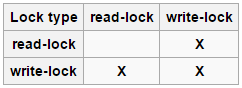
\includegraphics[width=0.4\linewidth]{figs/spm9/lockCompatibility.PNG}
\caption{Lock compatibilty table}
\label{fig:lockCompatibility}
\end{figure}

\begin{lstlisting}[caption=Eksemepl på Database transaction med DELETE]
BEGIN
	IF(checkIfdataCanDelete)
		BEGIN
			ROLLBACK;
		END
	ELSE
		BEGIN
			DELETE FROM [Table Name] WHERE [statement];
			COMMIT;
		END
END
\end{lstlisting}




